\documentclass[10pt]{beamer}

\setbeamersize{text margin left=0.5cm, text margin right=0.5cm}

\usepackage{alltt}%
%\usetheme{Boadilla}
\usetheme[progressbar = foot, background=light]{metropolis} 
%\useoutertheme{split}

%\usepackage{listings}
\makeatletter
\def\maxwidth{ %
  \ifdim\Gin@nat@width>\linewidth
    \linewidth
  \else
    \Gin@nat@width
  \fi
}
\makeatother

\definecolor{fgcolor}{rgb}{0.345, 0.345, 0.345}
\newcommand{\hlnum}[1]{\textcolor[rgb]{0.686,0.059,0.569}{#1}}%
\newcommand{\hlstr}[1]{\textcolor[rgb]{0.192,0.494,0.8}{#1}}%
\newcommand{\hlcom}[1]{\textcolor[rgb]{0.678,0.584,0.686}{\textit{#1}}}%
\newcommand{\hlopt}[1]{\textcolor[rgb]{0,0,0}{#1}}%
\newcommand{\hlstd}[1]{\textcolor[rgb]{0.345,0.345,0.345}{#1}}%
\newcommand{\hlkwa}[1]{\textcolor[rgb]{0.161,0.373,0.58}{\textbf{#1}}}%
\newcommand{\hlkwb}[1]{\textcolor[rgb]{0.69,0.353,0.396}{#1}}%
\newcommand{\hlkwc}[1]{\textcolor[rgb]{0.333,0.667,0.333}{#1}}%
\newcommand{\hlkwd}[1]{\textcolor[rgb]{0.737,0.353,0.396}{\textbf{#1}}}%
\let\hlipl\hlkwb

\usepackage{framed}
\makeatletter
\newenvironment{kframe}{%
 \def\at@end@of@kframe{}%
 \ifinner\ifhmode%
  \def\at@end@of@kframe{\end{minipage}}%
  \begin{minipage}{\columnwidth}%
 \fi\fi%
 \def\FrameCommand##1{\hskip\@totalleftmargin \hskip-\fboxsep
 \colorbox{shadecolor}{##1}\hskip-\fboxsep
     % There is no \\@totalrightmargin, so:
     \hskip-\linewidth \hskip-\@totalleftmargin \hskip\columnwidth}%
 \MakeFramed {\advance\hsize-\width
   \@totalleftmargin\z@ \linewidth\hsize
   \@setminipage}}%
 {\par\unskip\endMakeFramed%
 \at@end@of@kframe}
\makeatother

\definecolor{shadecolor}{rgb}{.97, .97, .97}
\definecolor{messagecolor}{rgb}{0, 0, 0}
\definecolor{warningcolor}{rgb}{1, 0, 1}
\definecolor{errorcolor}{rgb}{1, 0, 0}
\newenvironment{knitrout}{}{} % an empty environment to be redefined in TeX


\usepackage[utf8]{inputenc}
\usepackage{default}

\usepackage{xcolor}%for color mixing

\usepackage{amsmath}%
\usepackage{amsfonts}%
\usepackage{amssymb}%
\usepackage{graphicx}

\usepackage{tikz}
\usepackage{multirow}
\usepackage{booktabs}

\setbeamertemplate{itemize/enumerate body begin}{\small}

%%%%%%%%%%%%%%%%%%%%%%%%%%%%%%%%%%%%%%%%%%%%%%%%%%%%%%%%%%%%%%%%%%%%%%%%%%%%%%%%%%

\title{Statistical Modelling: Understanding Mean Structure}
\subtitle{Chapter 3}
\author{Timoth\'ee Bonnet and Terry Neeman}
\date{\today}

\begin{document}

%\lstset{language=R}%code

\AtBeginSection[]
{
  \begin{frame}<beamer>
    \frametitle{}
    \tableofcontents[currentsection,sectionstyle=show/show,subsectionstyle=show/shaded/hide]% down vote\tableofcontents[currentsection,currentsubsection,hideothersubsections,sectionstyle=show/hide,subsectionstyle=show/shaded/hide] 
  \end{frame}
}


\begin{frame}{}
\maketitle

\end{frame}
%%%%%%%%%%%%%%%%%%%%%%%


\begin{frame}{Key components of a statistical model of an experiment}
\begin{itemize}
  \item Outcome measure
  \begin{itemize}
   \item Response variable
   \item Measure of interest
  \end{itemize}
  \item Experimental factors 
  \begin{itemize}
   \item Conditions that can be manipulated 
   \item Conditions of interest (e.g. genotype, gender) 
   \item Main questions: do the conditions impact upon the outcome measure?
  \end{itemize}
  \item Blocking factors
  \begin{itemize}
   \item Conditions (not of interest) that may impact upon the outcome measure
   \item Sources of variation in the experiment that need to be controlled for
   \item Clustering of experimental units
  \end{itemize}
\end{itemize}

\vspace{0.2cm}
ALWAYS BEGIN WITH A RESEARCH QUESTION

\end{frame}
%%%%%%%%%%%%%%%%%%%%%%%

\begin{frame}{Simple linear models}
\centering
\Large
  ${\color{purple}{response}} = \underbrace{{\color{blue}{A}} + {\color{red}{D}} \times {\color{orange}{predictor}}}_{\substack{\text{Mean Structure} \\ \text{Experimental factors}}} + 
  \underbrace{{\color{gray}{\epsilon}}, \text{ with } {\color{gray}{\epsilon \sim N(0,\sigma)}}}_{\substack{\text{Variance Structure} \\ \text{Unrelated to experiment factors} \\ \text{Unexplained ``noise''}}}$

  
\end{frame}
%%%%%%%%%%%%

\begin{frame}{Example 1: Can drought tolerance in Arabidopsis be improved through genetic modification?}

\begin{block}{Context}
\begin{columns}
 \begin{column}{0.8\textwidth}
  Outcome measure: Leaf water retention LWR (\%)\\
  Experimental factors:
    \begin{itemize}
     \item Gene A, genotypes \texttt{(AA/aa)}
     \item Gene B, genotypes \texttt{(BB/bb)}
    \end{itemize}
   \end{column}
   \begin{column}{0.2\textwidth}
    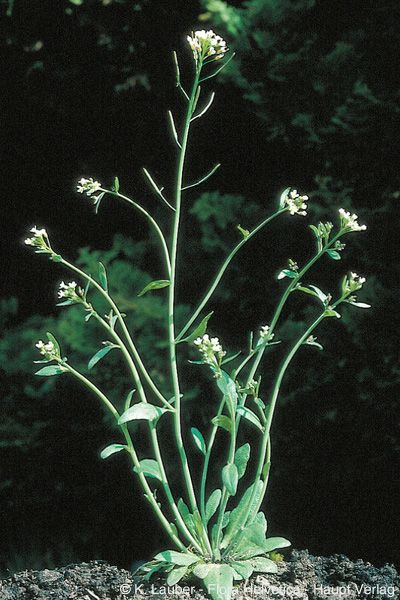
\includegraphics[width=0.7\textwidth]{Figures/arabid}
    
   \end{column}

   \end{columns}
   
\end{block}
How many parameters to describe the different genotypes combinations?
        
\pause

\begin{center}
\begin{tabular}{|l | l | l | l | }
\toprule
  \multicolumn{2}{|l|}{4 treatments} & \multicolumn{2}{l|}{Gene A}\\
  \cmidrule(lr){3-4}
  \multicolumn{2}{|l|}{}  & AA & aa\\
 	    \midrule
      Gene B & BB & $C$ & $C+A$\\
      \cmidrule(lr){3-4}
 	    & bb & $C+B$ & $C+A+B+D$\\
	    \bottomrule
  \end{tabular}
\end{center}
 
\end{frame}
%%%%%%%%%%%%%%

\begin{frame}{Two different models}

\textbf{Additive model - 3 parameters}
\begin{center}
\begin{tabular}{|l | l | l | l | }
\toprule
  \multicolumn{2}{|l|}{4 treatments} & \multicolumn{2}{l|}{Gene A}\\
  \cmidrule(lr){3-4}
  \multicolumn{2}{|l|}{}  & AA & aa\\
 	    \midrule
      Gene B & BB & $C$ & $C+A$\\
      \cmidrule(lr){3-4}
 	    & bb & $C+B$ & $C+A+B$\\
	    \bottomrule
  \end{tabular}
\end{center}
 

\textbf{Full factorial model / Interactive model  - 4 parameters }
\begin{center}
\begin{tabular}{|l | l | l | l | }
\toprule
  \multicolumn{2}{|l|}{4 treatments} & \multicolumn{2}{l|}{Gene A}\\
  \cmidrule(lr){3-4}
  \multicolumn{2}{|l|}{}  & AA & aa\\
 	    \midrule
      Gene B & BB & $C$ & $C+A$\\
      \cmidrule(lr){3-4}
 	    & bb & $C+B$ & $C+A+B+D$\\
	    \bottomrule
  \end{tabular}
\end{center}
 

 \textbf{\emph{What is different? What does the additive model assume?}}
\end{frame}
%%%%%%%%%%%%

\begin{frame}{Which model to use?}
 \textbf{Additive model - 3 parameters}
\begin{center}
\begin{tabular}{|l | l | l | l | }
\toprule
  \multicolumn{2}{|l|}{4 treatments} & \multicolumn{2}{l|}{Gene A}\\
  \cmidrule(lr){3-4}
  \multicolumn{2}{|l|}{}  & AA & aa\\
 	    \midrule
      Gene B & BB & $C$ & $C+A$\\
      \cmidrule(lr){3-4}
 	    & bb & $C+B$ & $C+A+B$\\
	    \bottomrule
  \end{tabular}
\end{center}
 

\textbf{Full factorial model / Interactive model - 4 parameters }
\begin{center}
\begin{tabular}{|l | l | l | l | }
\toprule
  \multicolumn{2}{|l|}{4 treatments} & \multicolumn{2}{l|}{Gene A}\\
  \cmidrule(lr){3-4}
  \multicolumn{2}{|l|}{}  & AA & aa\\
 	    \midrule
      Gene B & BB & $C$ & $C+A$\\
      \cmidrule(lr){3-4}
 	    & bb & $C+B$ & $C+A+B+D$\\
	    \bottomrule
  \end{tabular}
\end{center}
\end{frame}
%%%%%%%%%%%

\begin{frame}{Analysis in R}
 
 \begin{enumerate}
  \item Import data ''Prac3mockLWR.csv''
  \item Visualize data
  \item Model data
  \item Assess model assumptions
 \end{enumerate}

\end{frame}
%%%%%%%%%%%

\begin{frame}[fragile]{Analysis in R}
 
 1. Import data ``Prac3mockLWR.csv''
 
 \begin{knitrout}
\definecolor{shadecolor}{rgb}{0.969, 0.969, 0.969}\color{fgcolor}\begin{kframe}
\begin{verbatim}
  LWR <- read.csv("Prac3mockLWR.csv")
 \end{verbatim}
\end{kframe}
\end{knitrout}
 
\end{frame}
%%%%%%%%%%%

\begin{frame}[fragile]{Analysis in R}
 
2. Visualise the data

 \begin{knitrout}
\definecolor{shadecolor}{rgb}{0.969, 0.969, 0.969}\color{fgcolor}\begin{kframe}
\begin{verbatim}

ggplot(LWR, aes(GeneB,LWR,colour=GeneA)) +
  geom_boxplot() + geom_point()
 \end{verbatim}
\end{kframe}
\end{knitrout}
 
 Full factorial or additive?
 
\end{frame}
%%%%%%%%%%%



\begin{frame}[fragile]{Analysis in R}
 
3. Model data

 \begin{knitrout}
\definecolor{shadecolor}{rgb}{0.969, 0.969, 0.969}\color{fgcolor}\begin{kframe}
\begin{verbatim}
lmadditive <- lm(LWR ~ GeneA + GeneB, data = LWR)
summary(lmadditive)
anova(lmadditive)
 \end{verbatim}
\end{kframe}
\end{knitrout}

 \begin{knitrout}
\definecolor{shadecolor}{rgb}{0.969, 0.969, 0.969}\color{fgcolor}\begin{kframe}
\begin{verbatim}
lminteraction <- lm(LWR ~ GeneA * GeneB, data = LWR)
summary(lminteraction)
anova(lminteraction)
emmeans(lminteraction, pairwise ~ GeneA|GeneB)
emmeans(lminteraction, pairwise ~ GeneB|GeneA)
 \end{verbatim}
\end{kframe}
\end{knitrout}

What are the estimates for $A, B, C, D$ under each models?
\end{frame}
%%%%%%%%%%%



\begin{frame}[fragile]{Analysis in R}
 
4. Model assumptions

 \begin{knitrout}
\definecolor{shadecolor}{rgb}{0.969, 0.969, 0.969}\color{fgcolor}\begin{kframe}
\begin{verbatim}
plot(lminteraction)
 \end{verbatim}
\end{kframe}
\end{knitrout}

\end{frame}
%%%%%%%%%%%

\begin{frame}{Which cabbage cultivar has the higher Vitamin C content on average?}
 \begin{block}{Research context}
 \begin{columns}
  \begin{column}{0.8\textwidth}
   \begin{itemize}
    \item 60 cabbage heads
    \item 2 cultivars: c39 and c52
    \item 3 planting dates: Days 16, 20, 21
   \end{itemize}
  \end{column}
  \begin{column}{0.2\textwidth}
    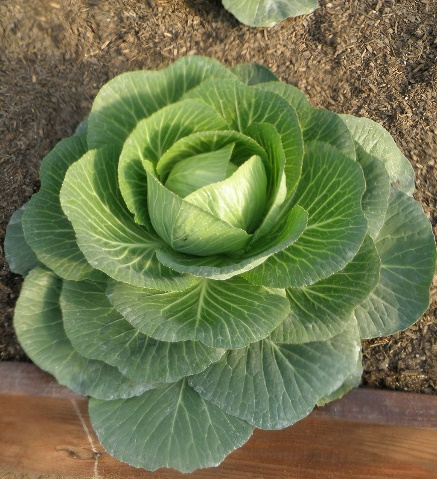
\includegraphics[width=0.9\textwidth]{Figures/cabbage}
  \end{column}

 \end{columns}
 \end{block}

 \only<1>{How many parameters to describe our scientific question?}
 
 \pause
 
 \begin{center}
\begin{tabular}{|l | l | l | l | }
\toprule
  \multicolumn{2}{|l|}{} & \multicolumn{2}{l|}{Cultivar}\\
  \cmidrule(lr){3-4}
  \multicolumn{2}{|l|}{}  & c39 & c52\\
 	    \midrule
      Planting& Day 16 & $A$ & $A+B$\\
 	 date   & Day 20 & $A+C$ & $A+B+C$\\
		& Day 21 & $A+D$ & $A+B+D$\\
		\midrule
\multicolumn{2}{|l|}{Marginal means} &  & \\	
	    \bottomrule
  \end{tabular}
\end{center}
 
\end{frame}
%%%%%%%%%%%%

\begin{frame}{Which cabbage cultivar has the higher Vitamin C content on average?}
 \textbf{Fit additive and interactive models in R}\\
 Dataset ``Prac3cabbagedata.csv''
\end{frame}
%%%%%%%%%%%%


\begin{frame}{Are temperature mechanisms modified in a genetically modified tomato plant?}
 \begin{block}{Research context}
 \begin{columns}
  \begin{column}{0.8\textwidth}
   \begin{itemize}
    \item 2 tomato plants
    \item 2 Genotypes: WT/mutant 
    \item Watering condition: Normal/Drought
    \item Leaf temperature measured
   \end{itemize}
  \end{column}
  \begin{column}{0.2\textwidth}
    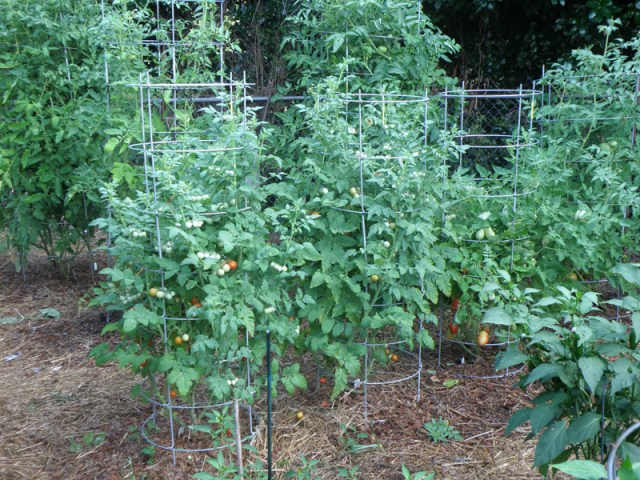
\includegraphics[width=0.9\textwidth]{Figures/tomato}
  \end{column}

 \end{columns}
 \end{block}
  \only<1>{How many parameters to describe our scientific question?}

   \pause
 
 \begin{center}
\begin{tabular}{|l | l | l | l | l |}
\toprule
  \multicolumn{2}{|l|}{} & \multicolumn{2}{l|}{Water condition} &\\
  \cmidrule(lr){3-5}
  \multicolumn{2}{|l|}{}  & Normal & Drought & Marginal means\\
 	    \midrule
      Genotype & WT &  & &\\
      \cmidrule(lr){2-5}
		& mutant &  & &\\
		\midrule
\multicolumn{2}{|l|}{Marginal means} &  & &\\	
	    \bottomrule
  \end{tabular}
\end{center}
 
\end{frame}
%%%%%%%%%%%

\begin{frame}{Are temperature mechanisms modified in a genetically modified tomato plant?}
 Dataset ``Prac3droughtdata.csv''\\
 Fit the appropriate model in R.\\
 Compare genotypes and water conditions with emmeans
 
\end{frame}
%%%%%%%%%%%

\begin{frame}{Relationship diameter/density differ between tree species?}
 
  \begin{block}{Research context}
 \begin{columns}
  \begin{column}{0.6\textwidth}
   \begin{itemize}
    \item \textit{Nothofagus} in the Andes
    \item 41 plots with 3 species (StandTypes)
    \item Outcome: Plot density
    \item Factors: StandType, QuadDiam
   \end{itemize}
  \end{column}
  \begin{column}{0.4\textwidth}
    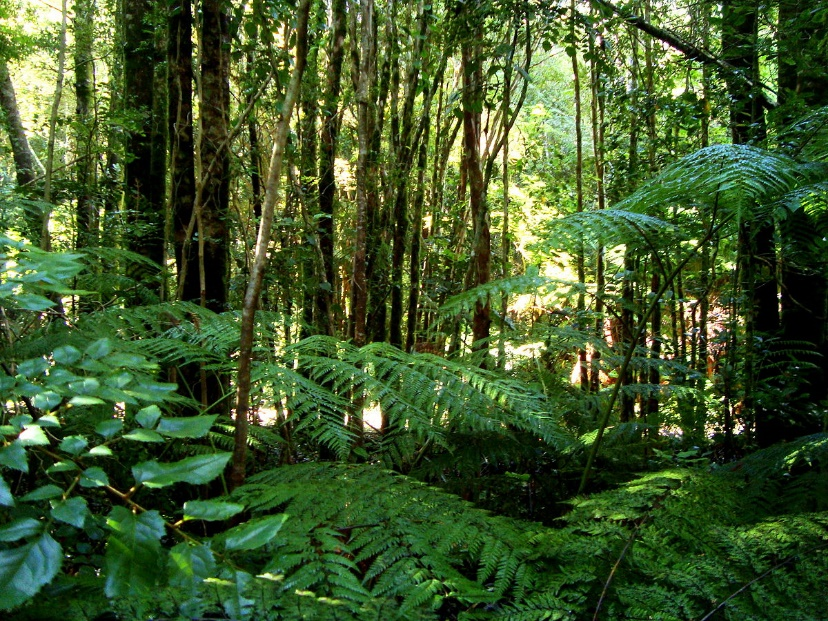
\includegraphics[width=0.7\textwidth]{Figures/forest}
  \end{column}

 \end{columns}
 \end{block}
 
 \pause
 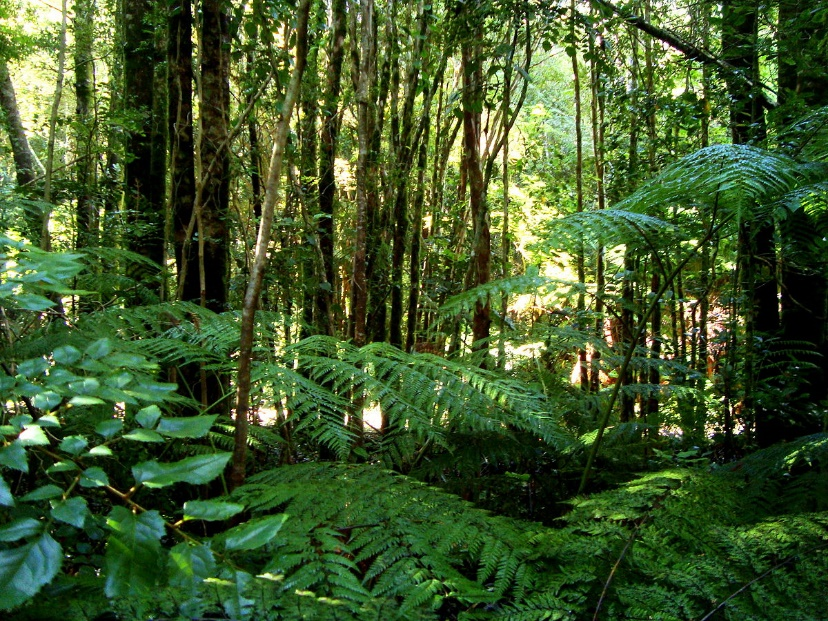
\includegraphics[width=0.7\textwidth]{Figures/trees}
 
\end{frame}
%%%%%%%%%%%

\begin{frame}{Which model to use}
 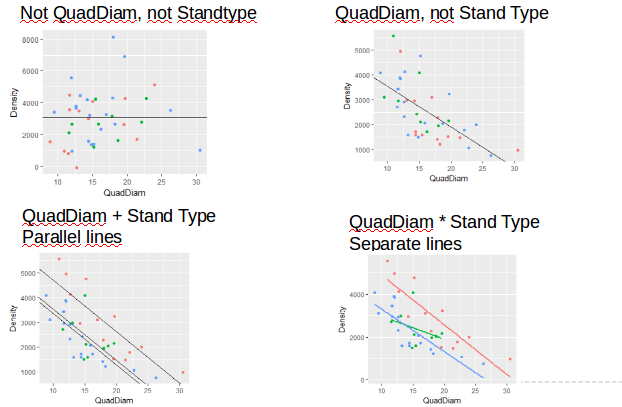
\includegraphics[width=0.8\textwidth]{Figures/tree4mod}
 
 Fit the models with ``Prac3forest.csv'' and answer the scientific question
\end{frame}
%%%%%%%%%%%%

\begin{frame}{Are NODk mice more susceptible to obesity when exposed to a high fat diet?}
  
  \begin{block}{Research context}
 \begin{columns}
  \begin{column}{0.5\textwidth}
   \begin{itemize}
    \item 37 mice: 16 NODk /21 WT
    \item Randomised to either regular or high fat diet
    \item Monitored for 14 weeks
    \item Outcome measure: Body weight (g)
    \item Experimental factors: Diet (2), Strain (2), Age (7)
   \end{itemize}
  \end{column}
  \begin{column}{0.5\textwidth}
    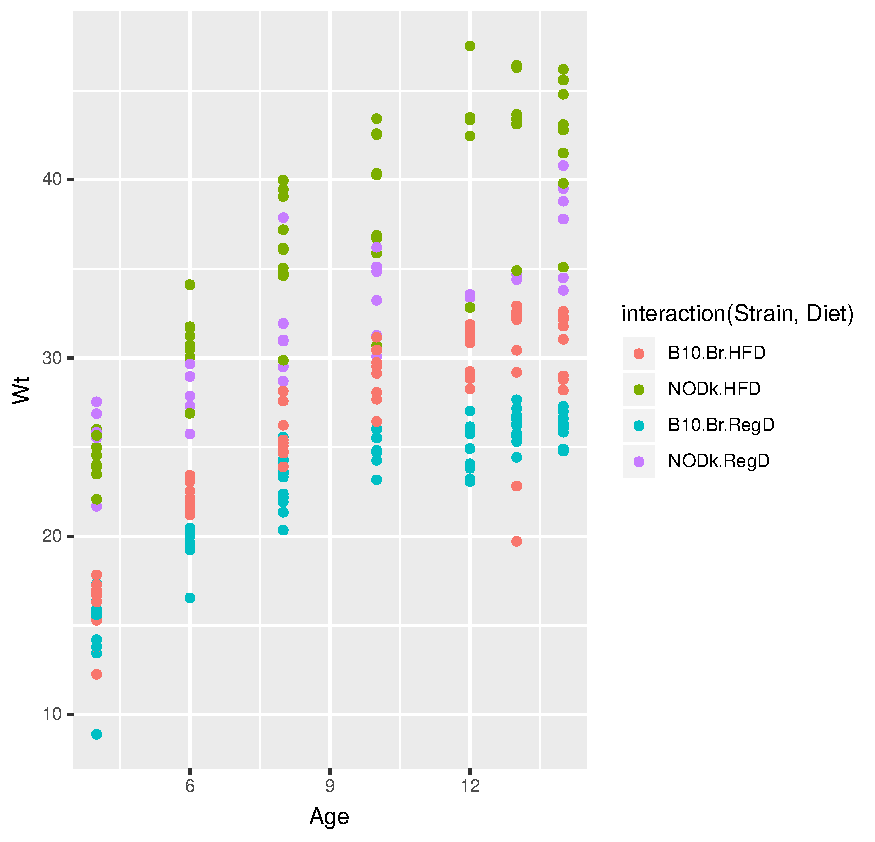
\includegraphics[width=\textwidth]{Figures/micedata}
  \end{column}

 \end{columns}
 \end{block}
 
 Data ``Prac3diabeticmice.csv''
 
\end{frame}
%%%%%%%%%%%


\end{document}
